\documentclass{training}

\title{3D Printing}
\date{\today}
\author{Blaise Thompson}

\begin{document}

\maketitle
\renewcommand{\baselinestretch}{0.5}\normalsize
\tableofcontents
\renewcommand{\baselinestretch}{1.0}\normalsize
\vfill

Part of the training materials prepared by the \href{https://shops.chem.wisc.edu/}{Chemistry Shops} at UW--Madison. \\
This document was prepared using \href{https://www.latex-project.org/}{\LaTeX}. \\
Source code and all associated files can be found at \href{https://git.chem.wisc.edu/shop/training/git}{git.chem/shop/training/git}. \\
If you find any mistakes or feel that any information is missing, please \href{https://git.chem.wisc.edu/shop/training/git/issues}{open an issue}. \\

\clearpage
\section{Options}

\begin{center}
\begin{tabular}{ l | l | l }
 material & cost & comment \\ \hline
 ABS & $\$5.00 / \mathrm{in}^3$ & self-service \\
 ASA & $\$3.50 / \mathrm{in}^3$ & via UW Makerspace \\
 PLA & $\$2.00 / \mathrm{in}^3$  & via UW Makerspace \\
 Nylon & ??? & via UW Makerspace. Scintillated.
\end{tabular}
\end{center}

To print via the UW Makerspace, contact Blaise Thompson.
A flat fee of $\$7$ will be added to the cost of material for any non self-service print.

\section{Self-Service Printing}

\begin{enumerate}
    \item Generate STL file, units mm. Bring to control computer.
    \item Turn on 3D printer.
    \item Ensure build plate is clean and correctly installed.
    \item Open Catalyst EX.
    \item File, Open STL.
    \item Choose layer resolution, interior fill.
    \item Pack. Note sum of model + support material volume. Bill yourself out.
    \item Print.
    \item On printer, press ``start model''.
    \item Wait until printer actually begins printing.
    \item If long print, leave ``This eqipment being used'' card.
    \item You are responsible for picking up your print.
\end{enumerate}

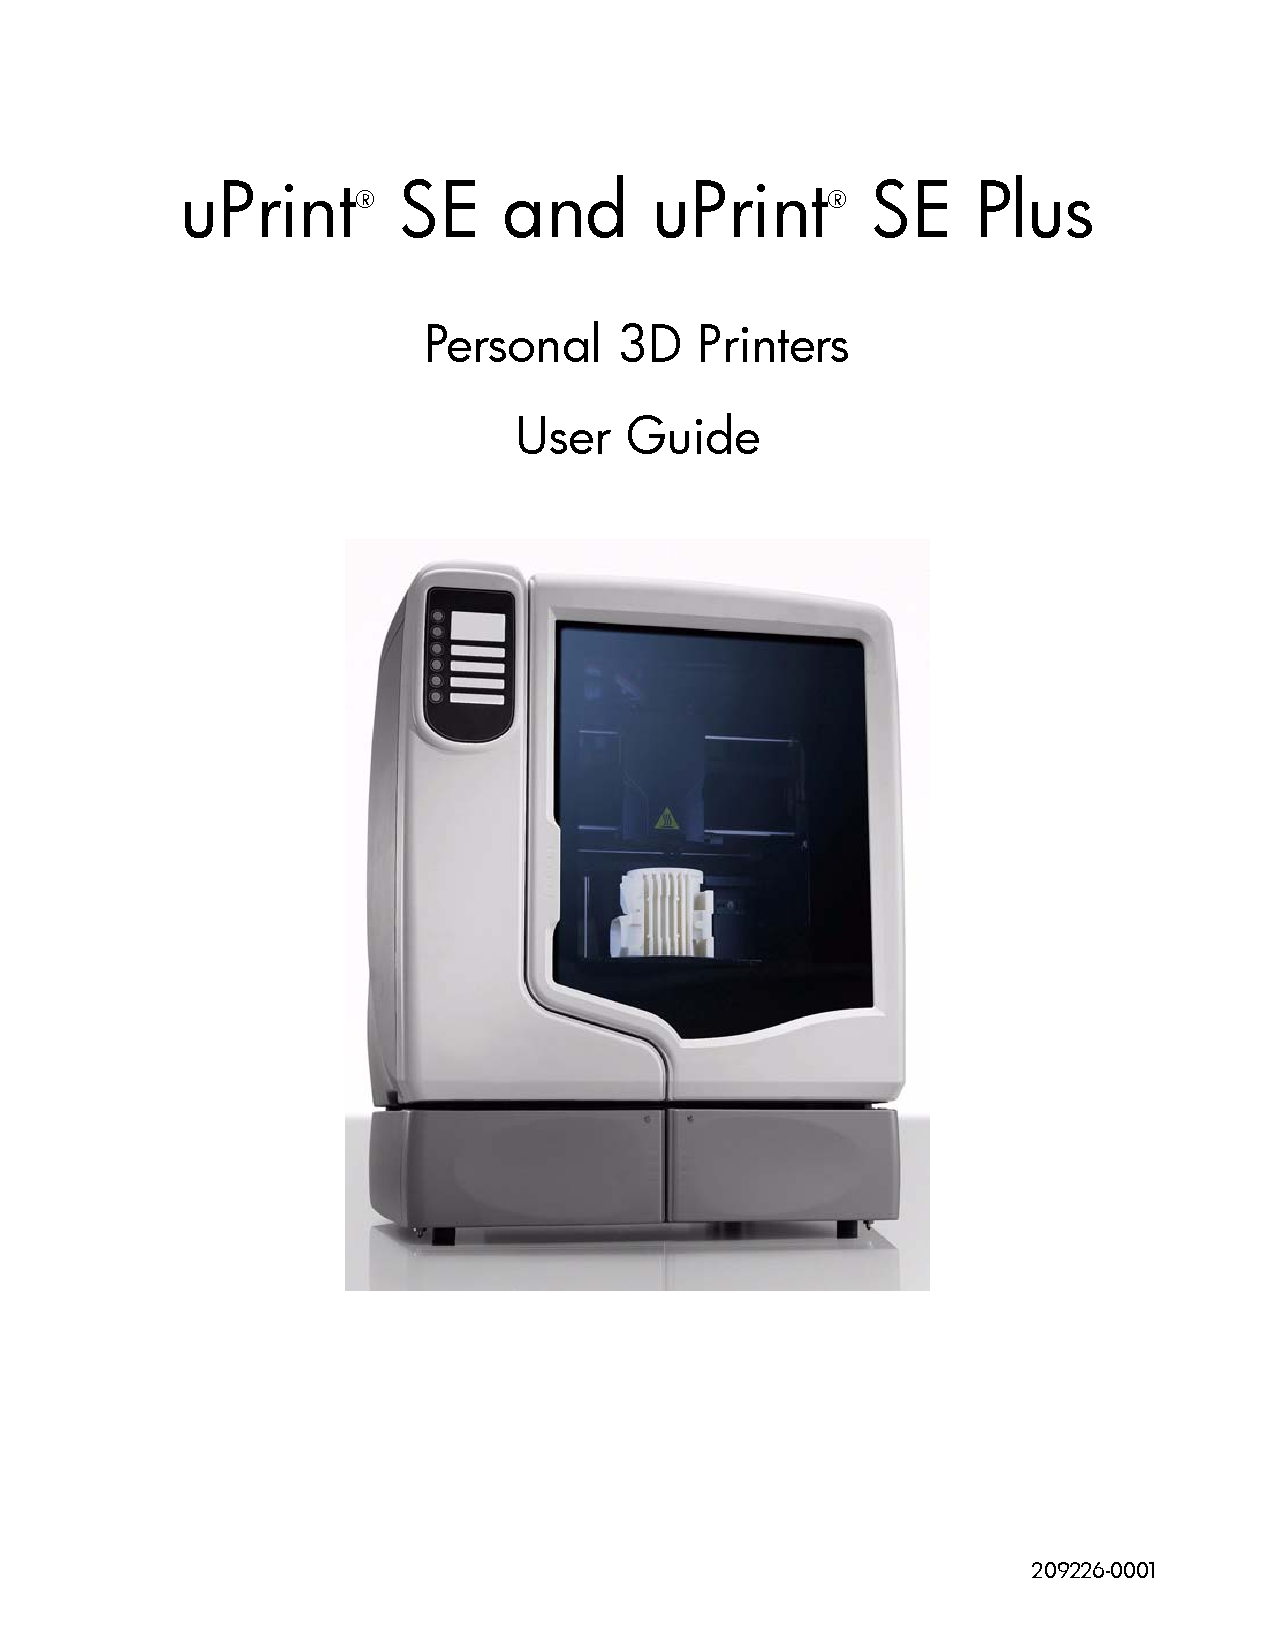
\includepdf[pages=-]{UprintSE_3Dprinter_Manual.pdf}

\end{document}
